\chapter{Data}

\textit{In this chapter we describe several potential datasets for digit recognition and hand-writing transcription. We use a more difficult version of the first dataset, MNIST, as a synthetic dataset for simulations. The real dataset for our task consist of the Swedish population records that are described in detail at the end of this chapter.}

% Here we describe some existing datasets for historical handwriting recognition and information extraction. We also consider their usefulness in regard to the thesis.

\section{MNIST}

The MNIST database contains 70,000 normalized images of handwritten digits \cite{MNIST_orig}.
%All images have the fix size $$ pixels.
Each image is represented by a floating-point matrix of $28 \times 28$, where the value $1.0$ corresponds to maximum presence of ink and $0.0$ corresponds to no ink.
The dataset is very popular for testing new algorithms and machine learning models \cite{MNIST}.
% It is even used for the introductory tutorial of Tensorflow \cite{}.
% https://www.tensorflow.org/get_started/mnist/pros
Although we can not use MNIST directly to evaluate the proposed models in this thesis, the dataset can be useful for quick simulations.
% and possibly also for pre-training a network as a prep.
In section \ref{sec:simulations} we present our findings by experimenting on a harder variation of MNIST.
We also initialize our experiments on the Swedish population records by a model that has been pre-trained on this harder variation of MNIST.

\section{Street View House Numbers}

The Street View House Numbers (SVHN) dataset consists of about 200,000 images of house numbers taken from Google Street View \cite{SVHN}. The dataset both contains original images of the house numbers as well as cropped and rescaled images for each digit. This dataset was used by \textcite{multidigit_streetview} to train models for transcribing a much larger dataset with millions of images. They could transcribe $83\%$ of the bigger dataset at $99\%$ accuracy.

\section{Datasets for historical handwriting recognition}

% TODO: line segmented not explained...
There are several publicly available databases of historical documents \cite{esposalles}: the George Washington, Parzival, Saint Gall, RODRIGO and GERMANA databases. The images are line segmented, that is the image has been divided into smaller segments so that each segment correspond to one line of text. The handwritten text on the line images has been transcribed.
% Several data of historical documents have been line segmented and transcribed for public use

Typically these datasets contain long documents of continuous text that differ significantly from civil population records, which are more structured and repetitive. Furthermore, each of these listed databases are written by one or two scribes, while we aim at understanding the handwriting of many scribes, which is necessary for indexing.
%They consist of long texts written by one or two scribes. In contrast, civil population records are typically written by many different scribes. Furthermore, civil population records are often structured, for example with columns and repetitive sentences.
% TODO add citations for each mentioned data set?

\section{Esposalles}
The Esposalles dataset consists of book indices and historical marriage licenses from the Cathedral of Barcelona \cite{esposalles}.
Experts have manually created \textbf{bounding boxes} around the words in the image so they can be separated into word images. Creating the bounding boxes for all words is also known as \textbf{word segmentation}.
% segmented all words to word images
The experts have also transcribed the text exactly as it occurs in each word image without spelling correction.

Although the Cathedral of Barcelona holds 291 books containing approximately 600,000 marriage licenses between 1451 and 1905, only a tiny fraction of this collection has been transcribed for the Esposalles dataset. The dataset consists of 173 pages from a single book written by a single scribe, containing 1747 marriage licenses between 1617 and 1619. Additionally, the dataset contains 29 pages of book indices.

The Esposalles dataset was used as ground truth for one of the tasks in the Robust reading competition at the International Conference on Document Analysis and Recognition (ICDAR) 2017\footnote{\url{http://rrc.cvc.uab.es/?ch=10&com=introduction}}.
For the competition, all words have been annotated with one of six categories such as
%the words have been annotated with semantic categories such as
surname of husband and surname of wife. The task was then to learn to recognize these categories automatically on new word images, which is known as \textbf{named entity recognition}.

We think that the exact transcriptions, bounding boxes and annotations make the dataset useful for
%segmentation-based methods in
tasks like word segmentation, handwriting recognition and named entity recognition.
Specifically for this thesis, we intend to classify years in a much larger range than 1617 to 1619 so the Esposalles dataset is simply too small. Furthermore, we are interested in exploring segmentation-free methods, so we would run on the entire input page rather than on the individual word images.

% TODO perhaps argue about slow and expensive process?
% We argue that creating a dataset of exact transcriptions and annotations by using paleographical experts is too slow and expensive to make a sufficiently large

%Furthermore, we believe that in order to make a system for fully automated indexing, the dataset needs to cover many more examples. Since using paleographical experts to transcribe and annotate each word is a slow and expensive process we do not expect the dataset to grow quickly.
% Thus, we assume that in order to create a sufficiently large dataset for training
%Thus we argue that for a dataset to grow sufficiently large it should
%1. not require the transcriber to be an expert and 2.
%only contain the most vital coarse information instead of every single word.


\section{IRIS}

While the Esposalles dataset focus on individual words transcribed by experts, the IRIS dataset contain record information extracted by volunteers in FamilySearch's indexing program \cite{Iris}.
Thus the extracted information does not contain exact transcriptions of the text but rather the most important semantic contents.
For examples, the indexer may have expanded abbreviations, replaced dittos with their intended values and ignored information that was deemed genealogically irrelevant.
% For example, abbreviations may have been expanded, dittos replaced by their intended values and information that was deemed genealogically irrelevant has been ignored.
Furthermore, while in Esposalles each transcribed word has a manually created bounding box, in IRIS there is no indication about what part of the image the information was extracted from.

The IRIS dataset consist of four collections of population records, totaling nearly 50,000 images.
% \paragraph{1, 2}
The first two collections in the IRIS dataset are the 1930 population census in the US and Mexico. The images consist of big tables with names and occupations in the cells.
For the purpose of this thesis where we extract the written year for each page, the 1930 censuses are not directly useful since they only contain records from a single year. Furthermore, it is not clear that if a system can learn from this collection that it would by useful for any other collection.
However, because the 1930 censuses are written on printed tables, word segmentation should be considerably simpler than for the free-form writing present in other collections.

% \paragraph{3}
The third collection contains marriage licenses between 1837-1944 in Arkansas. The marriage licenses are printed templates with handwritten text in the blanks.
It is likely that the system would learn to recognize the printed template and hence it would not be able to generalize to other collections that use different templates or free-form writing. If many collections were using the same template it would be useful to learn but then one might as well hard-code the positions of the blanks in the template. Thus, it is not very useful as training-data for models in this thesis.

% \paragraph{4}
The last collection contains more than 10,000 pages with records of baptisms, burials and marriages from French parishes between 1533-1906. Some of the pages contain printed templates but the majority seems to be free-form handwriting.
From manually inspecting these images, we conclude that many of them do not contain a written year anywhere on the page. These are problems that a future automated extraction system would need to handle, for this thesis however we settle for another dataset that seems somewhat easier.


\section{Swedish population records}

\begin{table}
\centering
\begin{tabular}{ l | r r r}
Name & Collection & Total images & Indexed images \\
\hline
Örebro	& 1647578	& 638873\footnote{\url{https://familysearch.org/search/collection/1647578}}	& 14330 \\
Uppsala	& 1647598	& 693757\footnote{\url{https://familysearch.org/search/collection/1647598}}	& 8869 \\
Södermanland	& 1647693	& 617735\footnote{\url{https://familysearch.org/search/collection/1647693}}	& 11827 \\
Kalmar	& 1930243	& 617325\footnote{\url{https://familysearch.org/search/collection/1930243}}	& 2081 \\
Jönköping	& 1930273	& 721027\footnote{\url{https://familysearch.org/search/collection/1930273}}	& 3637 \\
Västernorrland	& 1949331	& 273798\footnote{\url{https://familysearch.org/search/collection/1949331}}	& 2324 \\
\hline
Sum & & 3562515 & 43068
\end{tabular}
\caption{Collections of indexed Swedish records from FamilySearch.}
\label{tab:collections}
\end{table}


In cooperation with FamilySearch, we have been granted access to the extracted information from six collections of Swedish population records and their corresponding images.
% Each collection comes from a different region Sweden
Each collection contains records of baptisms, burials and marriages between 1607 and 1890 from many parishes within a specific Swedish region.
The regions, the number of images and the number of indexed images can be seen in table \ref{tab:collections}.
To our knowledge, this is the first time automated transcription or information extraction has been attempted on this dataset.
% These collections contain records of baptisms, burials and marriages in six regions between 1607 and 1890. They are the Swedish counterpart of the French IRIS collection mentioned above.


\begin{figure}
    \centering
    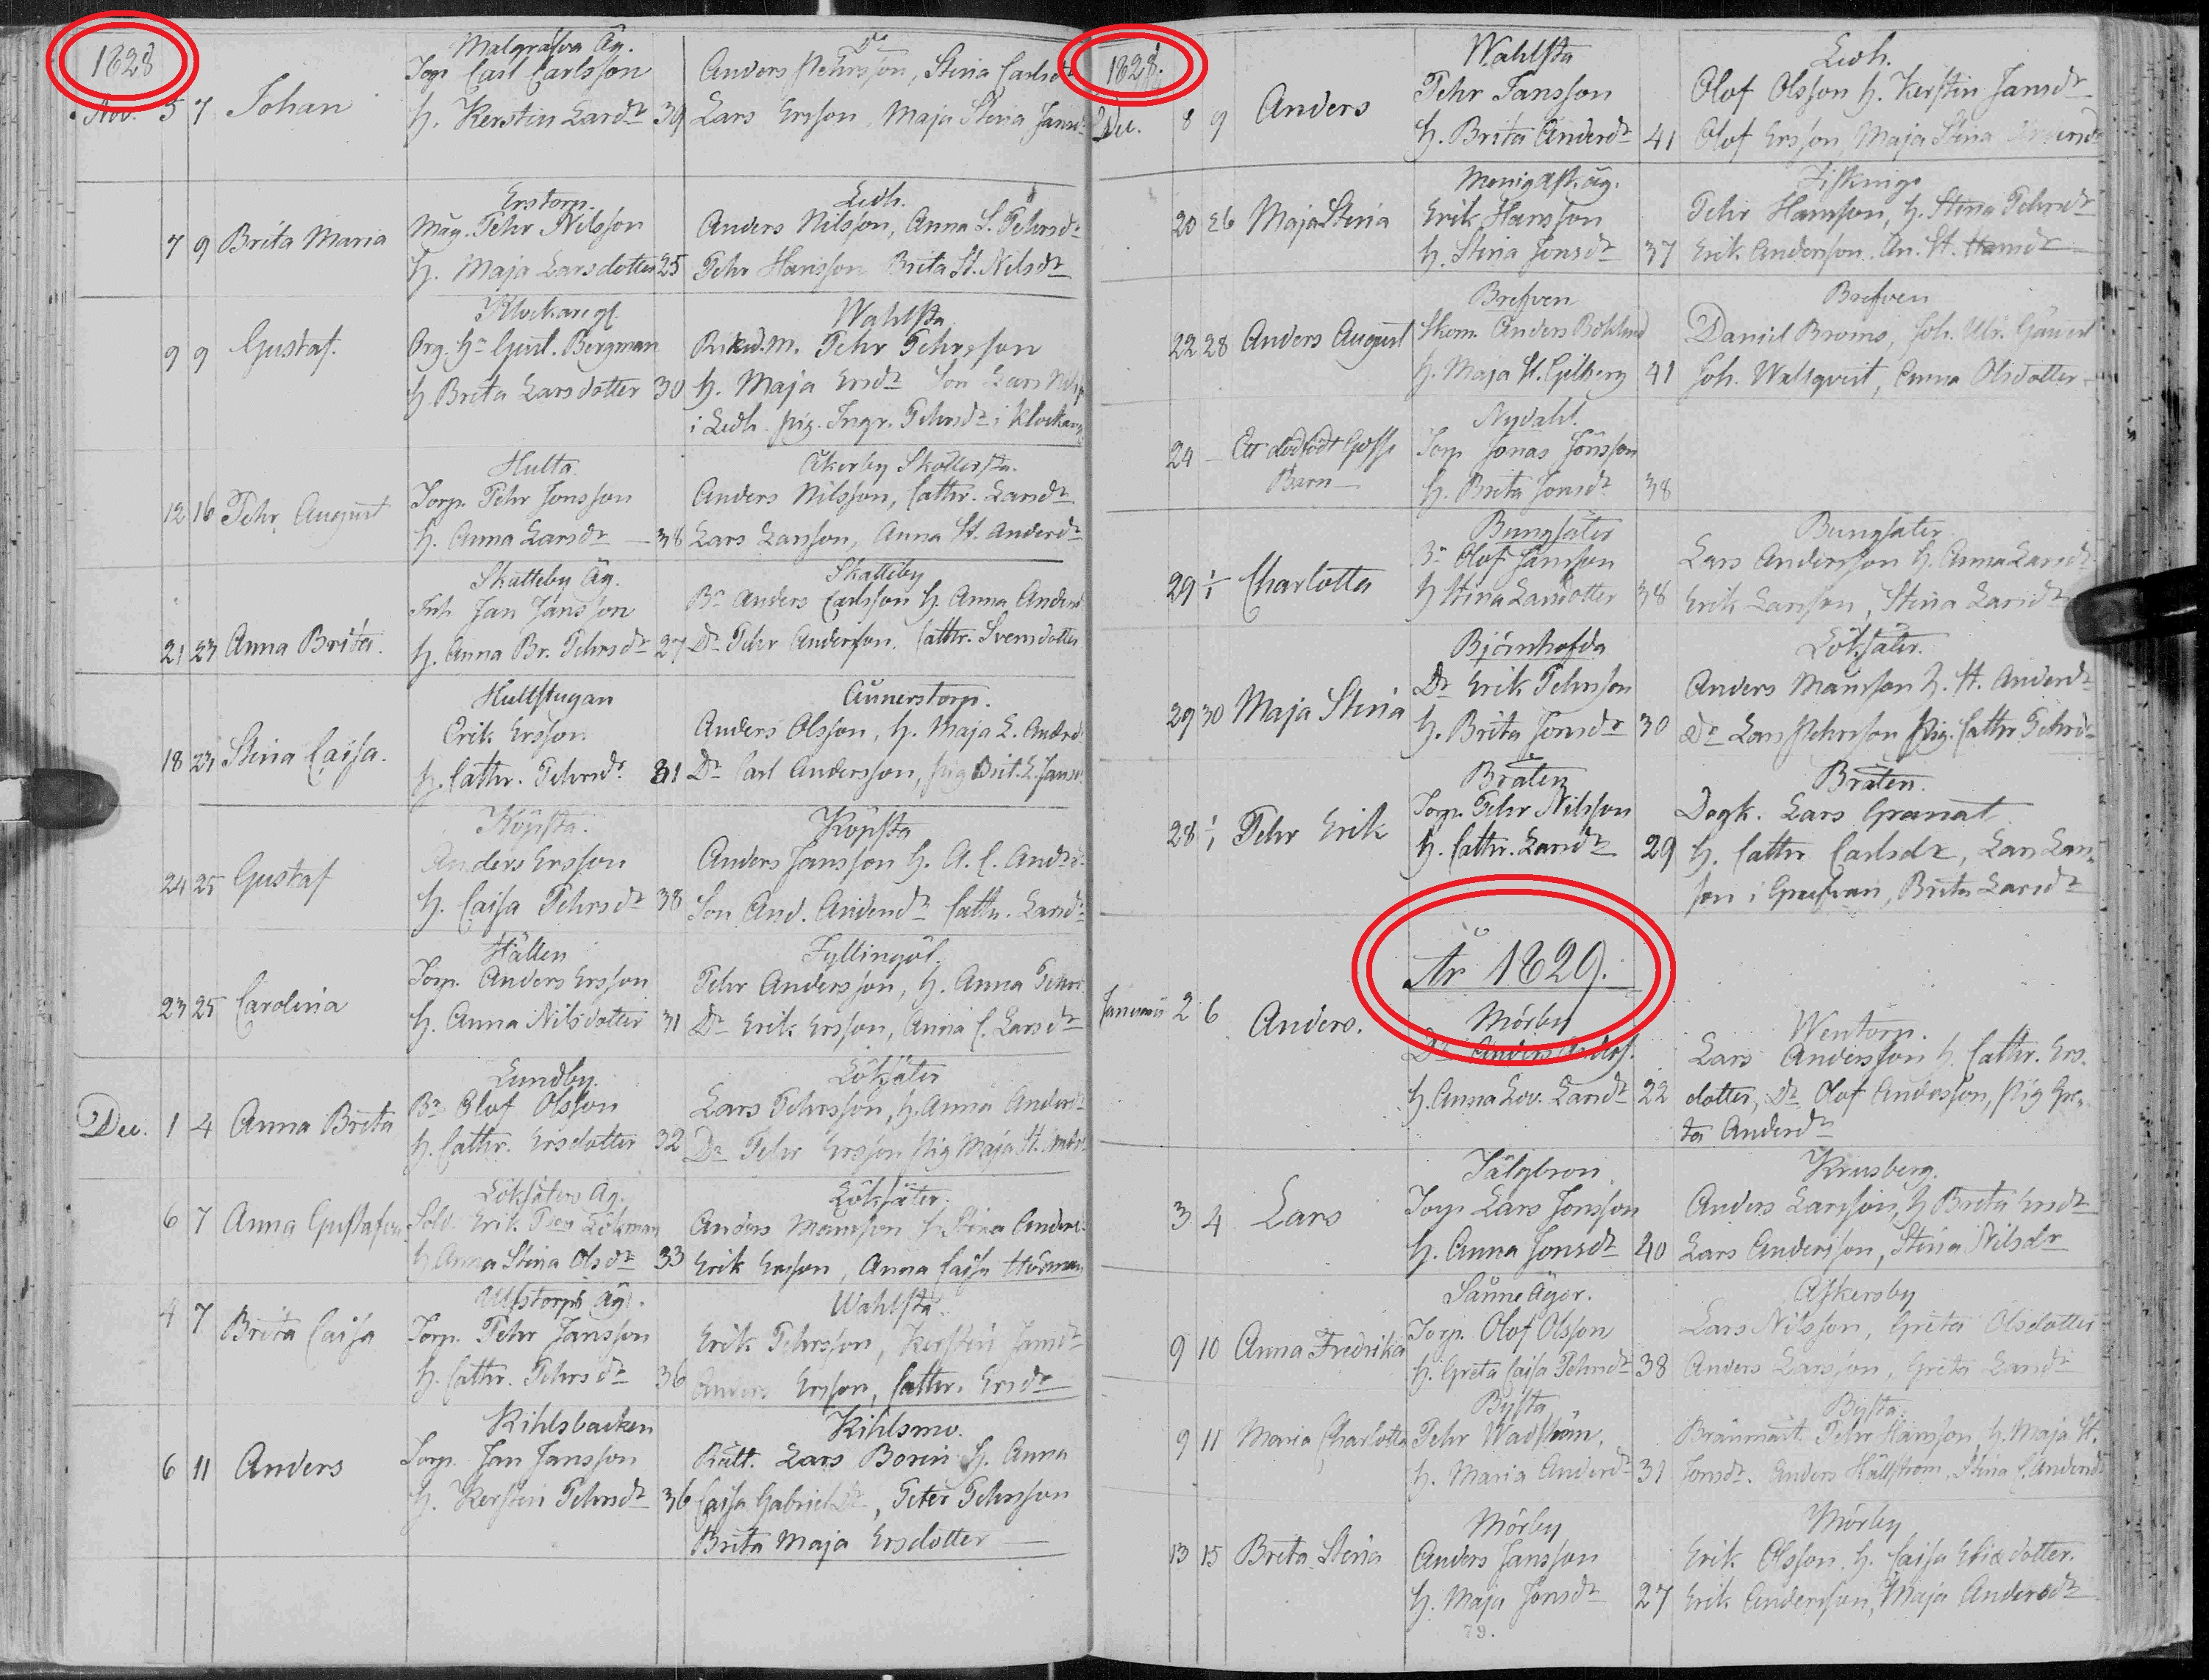
\includegraphics[scale=0.5]{resources/SWE_attention/S3HT-64P3-PQD.jpg}
    % \caption{Part of a page of burial records from the {\"O}rebro collection. Red lines have been added under the main years 1752 and 1753. There are also other years in the text such as 1687 and 1714 that we want to ignore. The picture is down-sampled to $25\%$.}
    \caption{Two pages of birth records from the book Asker C:4 in the Örebro collection. The main years, 1828 and 1829, have been emphasized with concentric ovals.}
    \label{fig:page}
\end{figure}


\subsection{The indexing process}

Just like with the IRIS dataset, the indexers have not provided us with bounding boxes or exact transcriptions but with extracted genealogical information. An indexed baptism record typically contains the name of the newborn child, the names of the parents, the date of birth, the date of baptism and location of the parents' home. The ecclesiastical records typically contain the names of witnesses to the baptism but this is ignored in the indexing process.

Each page is indexed by two independent volunteers. Any conflicts between the two versions is resolved by a third volunteer before submission.
The double work and review process increases the quality and consistency of the extracted information.
% Duplicating the indexing work and quality-checking increases the quality of the indexed data.
% Thus, the indexed information maintains a high quality even though it is not performed by professionals.

The extracted information is stored in the compressed GedcomX\footnote{\url{http://www.gedcomx.org/About.html}} format which has been developed specifically for genealogical information.
Each event of baptism, burial or marriage is stored as a record organized in the above mentioned six collections. Within a collection, the records do not seem to be stored in any particular order. Each record however contains information about which image it belongs to as well as some meta-information about the book the record comes from.

\subsection{Varying image size}

The images are stored in the JPG-format using lossy compression. Each image has a different size although the majority are about $5700 \times 4500$ pixels. There are also outliers with sizes like $7262 \times 5907$ pixels and $1885 \times 5110$ pixels. We think the varying image sizes is a result of cropping the image to fit the book in the photograph.
Since different books have different proportions, the aspect ratio of the images differs somewhat although it is often close to $1.25$:$1$.

\subsection{Page structure}

Most images consist of two pages, which are always handwritten. Sometimes the pages have pre-printed headers and vertical lines for columns, other times they are entirely free-form.
The year can often be found near the top of the page, either to the left or in the middle. See figure \ref{fig:page} for an example.


\begin{figure}
    \centering
    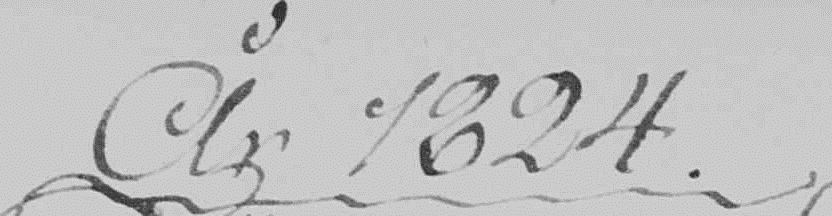
\includegraphics[scale=0.3]{resources/ar_kalmar/ar1824.png}
    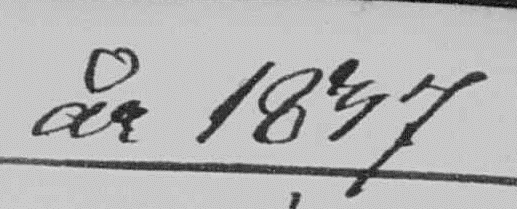
\includegraphics[scale=0.3]{resources/ar_kalmar/ar1837.png}
    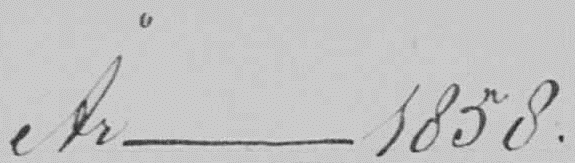
\includegraphics[scale=0.3]{resources/ar_kalmar/ar1858.png}
    \caption{Three variations of the word \textquote{\r{a}r} in page headers in the Kalmar collection.}
    \label{fig:aar}
\end{figure}


Although the general structure is the same for all six collections, the exact page layout differs greatly both within and between collections. Another difference that may be relevant for our model is that sometimes the year is following the word \textquote{\r{a}r}, although the handwriting style for the word can be very different depending on time and place; see figure \ref{fig:aar} for some examples.


\subsection{Multiple years per page} \label{sssec:swe_multiyear}

 % Additionally, when the year changed the scribe often indicated so by writing the new year in big letters before the block of new records.
Typically, the scribes did not use a new page for every new year but indicated the change of year by writing the new year in big letters before continuing to write the new records; an example of this can be seen in Figure \ref{fig:page}.
Thus besides at the top, written years can be found in virtually any part of the page. Another consequence is that a page can contain several years in a sequence like $\langle 1771, 1772, 1773, 1774 \rangle$. This is especially true for small parishes where there may not have been so many burials per year. Out of the 43,068 indexed images, 16,074 or $37.3\%$ have more than one year in the extracted information. There are also cases where the page span several years but with a small gap: $\langle 1771, 1773, 1774 \rangle$.

Some images however do not contain a written year, the year is simply implied from previous pages. For such instances, indexers are instructed to search the previous and following image for an indication of the year. If the implied year is found, it is noted in the extracted information, otherwise it is indicated as unknown.
If the year is unknown or the image is blank, we ignore the image because we do not have a label for it and we expect that the year is anyway not indicated in the image. Of the indexed images, $471$, or $1\%$, have no year label.

However, in the extracted information there is no way to distinguish whether the extracted year came from the same image or if it was implied from a neighboring image. Thus, it is inevitable that some images in the dataset have labels although the year is actually not written in the image. One way to counter this problem would be to only train on images that are labeled with more than one year, expecting an indicated year change somewhere in the image. Doing so would however reduce the dataset to $37.3\%$ of the original size.
Although we have no way to calculate how often the label implies a year that is missing from the image without manually inspecting every image, we assume that it is relatively rare and thus negligible.

Another kind of false labels are years occurring in free-form text. For example, a page with burial records for 1771 may mention that a deceased person was born in 1725. In this case, we only want to recognize 1771 although 1725 is actually another year present in the image.

\subsection{Partioning}

We divided the dataset into three partitions, one training set, one main test set and another test set for generalizing to new unseen scribes and books.

The images in the four largest collections (Örebro, Uppsala, Södermanland and Jönköping) were independently randomly selected to belong to the training set, with $90\%$ probability, or to the main test set, with $10\%$ probability.
Thus the training set and the main test set are disjoint, but are drawn from the same books and scribes. Therefore, we can use the main test set to detect overfitting of specific images.
The training set consists of 34,623 labeled images and the and the main test set of 4040 images.
% The remaining four collections were divided into training and testing by randomly


% The other test set however comes from entirely different regions and new scribes whose handwriting has not been seen by the model before. We can therefore use the test set to detect overfitting on specific images while the validation set can measure how well the model generalizes to new books and regions as in a realistic use case scenario.

The two smallest collections (Kalmar and Västernorrland) were reserved entirely for the second test set. The model has never been trained on recognizing handwriting from these scribes and may also be unfamiliar to page layouts used in these regions. Thus we can measure how well the model generalizes to new books and regions as in a realistic use case scenario. However, there is a possible caveat that these regions have been less indexed by volunteers because they are more difficult to read than the other four and hence may produce overly pessimistic results.

%We want to investigate how well learning in some regions can generalize to other regions. We also want to reserve these collections to validate any potential scheme for post-processing since we expect that a sequence of pages will correspond to a mostly unbroken sequence of years.

%The four largest collections have each been randomly divided into a training set ($90\%$) and a test set ($10\%$). The combined training set thus consist of $34623$ labeled images and the test set of $4040$ images.

\subsection{Label density} \label{sssec:few_labels}

Some labels occur very few times in the dataset. Although the labels span from 1607 to 1890, the majority of images lie between 1690 and 1861, with very few examples outside. Each year occurs in 147 images on average and few of the labels have more than 300 examples in the combined training and test data.
In this counting, we give each image a weight of one, so for multiyear images, we increment the count for each year in the label by a fraction of one.
